\documentclass[12pt]{article}
\usepackage{graphicx} % For including graphics
\usepackage{amsmath,amsfonts,amssymb} % For mathematical symbols
\usepackage{hyperref} % For hyperlinks
\usepackage{listings} % For including code
\usepackage{color} % For coloring code
\usepackage{geometry}
\geometry{letterpaper, portrait, margin=1in}

\definecolor{codegreen}{rgb}{0,0.6,0}
\definecolor{codegray}{rgb}{0.5,0.5,0.5}
\definecolor{codepurple}{rgb}{0.58,0,0.82}
\definecolor{backcolour}{rgb}{0.95,0.95,0.92}

\lstdefinestyle{mystyle}{
    backgroundcolor=\color{backcolour},   
    commentstyle=\color{codegreen},
    keywordstyle=\color{magenta},
    numberstyle=\tiny\color{codegray},
    stringstyle=\color{codepurple},
    basicstyle=\footnotesize\ttfamily, % This applies the monospace font
    breakatwhitespace=false,         
    breaklines=true,                 
    captionpos=b,                    
    keepspaces=true,                 
    numbers=left,                    
    numbersep=5pt,                  
    showspaces=false,                
    showstringspaces=false,
    showtabs=false,                  
    tabsize=2
}


\lstset{style=mystyle}

\title{ELCT 562 CA6}
\author{Jacob Vaught}
\date{\today}

\begin{document}

\maketitle

\section{Problem Statement}
Let \(E_s/N_0 \in \{0, 2, 4, \ldots, 20\} \text{ dB}\) for normalized 16-QAM constellations (i.e., \(E_s = 1\)):
\begin{enumerate}
    \item Plot the constellation points in the complex plane.
    \item For a given \(E_s/N_0\):
    \begin{itemize}
        \item[a.] Generate 100000 random data symbols in MATLAB where the points are equally likely.
        \item[b.] Add AWGN noise to the generated symbols.
        \item[c.] Develop a detector based on maximum likelihood.
        \item[d.] Calculate the symbol-error rate (SER) with the experiment.
    \end{itemize}
    \item Plot SER versus \(E_s/N_0\) curve in MATLAB.
    \item Plot theoretical SER versus \(E_s/N_0\) curve on the same figure and compare.
\end{enumerate}
\newpage
\section{16-QAM Constellation}
The 16-QAM constellation maps the data symbols onto the complex plane as shown in Figure \ref{fig:constellation}. Grey-Coding was not used in this simulation, although it would be a trivial task to implement.

\begin{figure}[htbp]
\centering
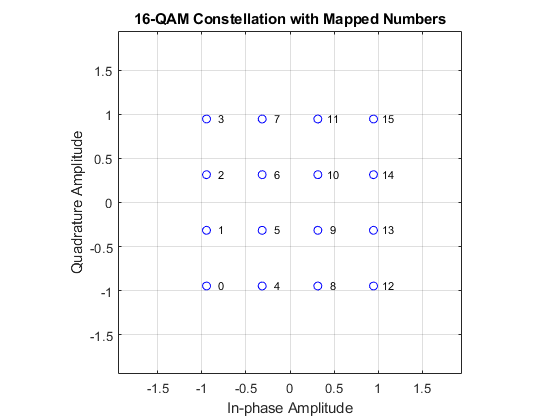
\includegraphics[width=0.8\textwidth]{b.png}
\caption{16-QAM Constellation with Mapped Numbers}
\label{fig:constellation}
\end{figure}
\newpage
\section{Symbol Error Rate (SER)}
The SER performance of the 16-QAM system is depicted in Figure \ref{fig:ser} both theoretically and through simulation.

\begin{figure}[htbp]
\centering
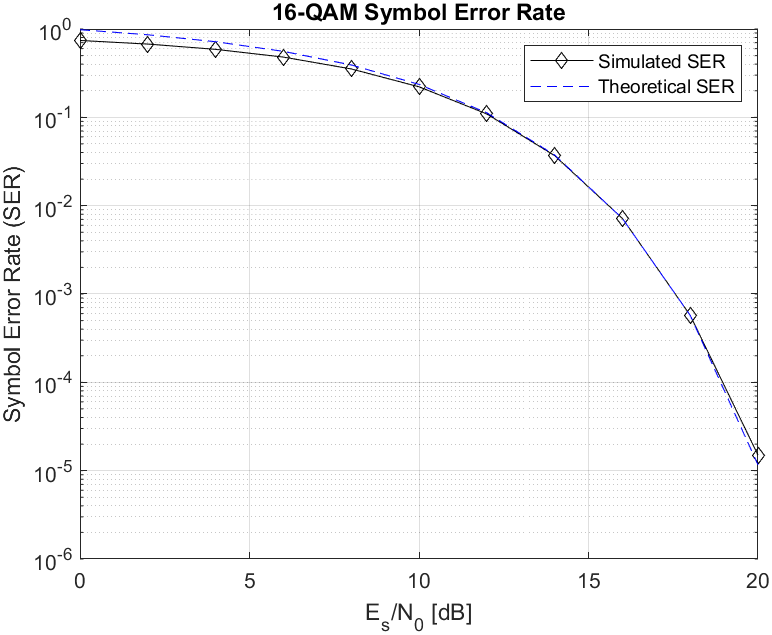
\includegraphics[width=0.9\textwidth]{a.png}
\caption{16-QAM Symbol Error Rate}
\label{fig:ser}
\end{figure}
\newpage
\section{MATLAB Explanation }

\subsection{Initial Setup and Symbol Generation}
The MATLAB code starts by clearing the environment and defining initial parameters for the simulation. `N` represents the number of symbols to be generated, and `EsN0\_dB` is a range of $E_s/N_0$ values in dB.

\begin{lstlisting}[language=Matlab]
clear; close all; clc;
N = 1000000; % Number of symbols
EsN0_dB = 0:2:20; % From 0 to 20 dB
data_symbols = randi([0, 15], N, 1); % Generate 16-QAM symbols
\end{lstlisting}

This snippet initializes variables and generates $10^6$ random data symbols for 16-QAM modulation, where each symbol can be any integer between 0 and 15.

\subsection{Mapping to 16-QAM Constellation}
Symbols are mapped to their respective positions in the 16-QAM constellation. This is achieved through the `map16QAM` function, which calculates the in-phase (I) and quadrature (Q) components and applies a scaling factor for normalization.

\begin{lstlisting}[language=Matlab]
[I, Q, scaling_factor] = map16QAM(data_symbols);
symbols = I + 1j * Q; % Combine I and Q into complex symbols
\end{lstlisting}

This function divides the symbols into I and Q components, normalizing them so that the average symbol energy $E_s = 1$.

\subsection{Transmission Over AWGN Channel}
The `simulateAWGNchannel` function simulates the transmission over an AWGN channel, adding noise to the symbols based on the $E_s/N_0$ values. It then detects the symbols and calculates the Symbol Error Rate (SER).

\begin{lstlisting}[language=Matlab]
SER = simulateAWGNchannel(N, symbols, data_symbols, EsN0_dB, scaling_factor);
\end{lstlisting}

This function adds noise to each symbol and uses a maximum likelihood approach to detect the transmitted symbols from the received noisy symbols. The SER is computed for each $E_s/N_0$ value.

\subsection{Plotting SER and Displaying Constellation}
The SER versus $E_s/N_0$ curve and the 16-QAM constellation are visualized using `plotSER` and `display16QAMConstellation` functions, respectively.

\begin{lstlisting}[language=Matlab]
plotSER(EsN0_dB, SER); % Plot SER
display16QAMConstellation(scaling_factor); % Display constellation
\end{lstlisting}

`plotSER` generates a graph of the simulated and theoretical SER against $E_s/N_0$. `display16QAMConstellation` plots the 16-QAM constellation with mapped numbers.

\subsection{map16QAM Function}
This function maps integer data symbols to their corresponding points in the 16-QAM constellation. It takes the data symbols as input and returns their in-phase (I) and quadrature (Q) components, along with a scaling factor to ensure the average symbol energy \(E_s = 1\).

\begin{lstlisting}[language=Matlab]
function [I, Q, scaling_factor] = map16QAM(data_symbols)
    I = mod(data_symbols, 4) * 2 - 3; % In-phase component
    Q = floor(data_symbols / 4) * 2 - 3; % Quadrature component
    scaling_factor = 1 / sqrt(10); % Normalize for average energy Es = 1
    I = I * scaling_factor;
    Q = Q * scaling_factor;
end
\end{lstlisting}

The I and Q components are derived from the modulo and integer division of the original data symbols, respectively. The constellation is scaled so that the average symbol energy equals one, which is necessary for comparing different modulation schemes under the same energy conditions.

\subsection{simulateAWGNchannel Function}
This function simulates the effect of an Additive White Gaussian Noise (AWGN) channel on the transmitted symbols. It computes the Symbol Error Rate (SER) for different \(E_s/N_0\) values.

\begin{lstlisting}[language=Matlab]
function SER = simulateAWGNchannel(N, symbols, data_symbols, EsN0_dB, scaling_factor)
    SER = zeros(length(EsN0_dB), 1);
    for k = 1:length(EsN0_dB)
        N0 = 1 / (10^(EsN0_dB(k) / 10));
        noise = sqrt(N0/2) * (randn(N, 1) + 1j*randn(N, 1));
        received_symbols = symbols + noise;
        detected_symbols = detectSymbols(received_symbols, scaling_factor);
        SER(k) = sum(data_symbols ~= detected_symbols) / N;
    end
end
\end{lstlisting}

For each \(E_s/N_0\) value, this function calculates the noise power \(N_0\), generates corresponding noise, and adds it to the transmitted symbols. It then calls `detectSymbols` to detect the transmitted symbols from the noisy received symbols, calculating the SER by comparing the detected symbols to the original data symbols.

\subsection{detectSymbols Function}
The `detectSymbols` function is a maximum likelihood detector. It decides which constellation point is closest to the received symbol and maps the received symbol to that constellation point.

\begin{lstlisting}[language=Matlab]
function detected_symbols = detectSymbols(received_symbols, scaling_factor)
    constellation = scaling_factor * [-3, -1, 1, 3];
    N = length(received_symbols);
    detected_symbols = zeros(N, 1);
    for n = 1:N
        distances = abs(received_symbols(n) - (constellation.' + 1j * constellation));
        [~, minIndex] = min(distances(:));
        detected_symbols(n) = minIndex - 1;
    end
end
\end{lstlisting}

This function calculates the Euclidean distance between each received symbol and all possible constellation points. The index of the nearest constellation point is then mapped back to the corresponding data symbol.

\subsection{plotSER Function}
The `plotSER` function plots both the simulated and theoretical Symbol Error Rates (SER) against \(E_s/N_0\) for the 16-QAM modulation scheme.

\begin{lstlisting}[language=Matlab]
function plotSER(EsN0_dB, SER)
    theoretical_SER = 3 * qfunc(sqrt(0.2 * (10.^(EsN0_dB / 10))));
    figure;
    semilogy(EsN0_dB, SER, 'kd-', 'DisplayName', 'Simulated SER');
    hold on;
    semilogy(EsN0_dB, theoretical_SER, 'b--', 'DisplayName', 'Theoretical SER');
    grid on; xlabel('E_s/N_0 [dB]'); ylabel('Symbol Error Rate (SER)');
    ylim([1e-6, 1]); legend('show'); title('16-QAM Symbol Error Rate');
end
\end{lstlisting}

This function uses the Q-function to calculate theoretical SER values for comparison with the simulated SER. It then plots both sets of values on a semi-logarithmic scale to assess the performance of the 16 QAM modulation under different signal-to-noise ratios.

\subsection{display16QAMConstellation Function}
This function visualizes the 16-QAM constellation map, showing how data symbols are mapped to specific I (In-phase) and Q (Quadrature) values in the complex plane. This aids in understanding the modulation scheme's structure.

\begin{lstlisting}[language=Matlab]
function display16QAMConstellation(scaling_factor)
    constellation_points = scaling_factor * [-3 -1 1 3];
    [X, Y] = meshgrid(constellation_points, constellation_points);
    constellation_symbols = X + 1j * Y;
    constellation_symbols = constellation_symbols(:);
    figure;
    plot(real(constellation_symbols), imag(constellation_symbols), 'bo');
    text(real(constellation_symbols) + 0.1, imag(constellation_symbols), num2str([0:15]'), 'FontSize', 8);
    grid on; axis equal; title('16-QAM Constellation with Mapped Numbers');
    xlabel('In-phase Amplitude'); ylabel('Quadrature Amplitude');
    xlim([min(real(constellation_symbols))-1, max(real(constellation_symbols))+1]);
    ylim([min(imag(constellation_symbols))-1, max(imag(constellation_symbols))+1]);
end
\end{lstlisting}

This function generates a grid of constellation points scaled according to the specified `scaling\_factor`, ensuring the average energy of the constellation is normalized. It then plots these points on a 2D plane, marking each with its corresponding digital symbol (from 0 to 15), making it easier to visualize the digital-to-analog mapping process inherent in 16-QAM modulation.

\end{document}